\documentclass[12pt]{article}
\renewcommand{\baselinestretch}{1.5}
\usepackage[OT4]{fontenc}
\newtheorem{define}{Definition}
\usepackage{amsmath}
\usepackage{graphicx}
\usepackage{enumitem}
\usepackage{float}

\oddsidemargin=0.15in
\evensidemargin=0.15in
\topmargin=-.5in
\textheight=9in
\textwidth=6.25in

\setlength{\oddsidemargin}{.25in}
\setlength{\evensidemargin}{.25in}
\setlength{\textwidth}{6in}
\setlength{\topmargin}{-0.4in}
\setlength{\textheight}{8.5in}

\newcommand{\handout}[5]{
	\noindent
	\begin{center}
		\framebox{
			\vbox{
				\hbox to 5.78in { {\bf #1}
					\hfill #2 }
				\vspace{4mm}
				\hbox to 5.78in { {\Large \hfill #5  \hfill} }
				\vspace{2mm}
				\hbox to 5.78in { {\it #3 \hfill #4} }
			}
		}
	\end{center}
	\vspace*{4mm}
}

\newcommand{\header}[3]{\handout{NUS CS-3235: Computer Security}{\today}{Lecturer: Reza Shokri}{Student: #2\quad#3}{#1}}

%======================================
%======================================
%======================================

\begin{document}

% Indicate your name and your student number here (e.g., A01xxx)
\header{Assignment 3 Report}{Wang Chenyu}{A0245095B}
\section{Overview}

Although the traffic data are encrypted, we can still find some "patterns" of the traffic data and then it is able for us to "distinguish" then. By "summarising" the traffic data and then using machine learning and apply "Classification Algorithm", urls can be classified properly.

\section{Implementation Mechanism}

In general, we need to figure out two important things:
\begin{enumerate}
  \item What classification algorithms shall we use?
  \item How can we "abstract summary from each url file?"
\end{enumerate}

The first question gets multiple answers: Logistic Regression, k-Nearest Neighbors, Decision Trees, Support Vector Machine, Naive Bayes... However, in order to find the best one, we need to know what the algorithm needs to perform:  
\begin{enumerate}
  \item Many features as input.
  \item Multiple ( 35 ) label classes as output.
\end{enumerate}

So our remaining choices are SVM, KNN and Naive Bayes because they can deal with classifications with multiple output labels well. Then after reading some papers about network analysis, I planned to try KNN and SVM. It turned out that KNN(90\%) works better with SVM(40\%), I think the reason is that: if you have k different features, then SVM will try to set up hyper-planes as "boundaries" to divide the data and when you put a point inside to predict, the result is which "Section" the point lands to. It is indeed very good in some cases, however because the inputs are all 'network traffic' features, they are quite similar and do not have such a clear "boundary" to differ them, so SVM may not work well. 

Different with SVM, KNN will let the k nearest neighbours of the test point to 'Vote' in order to determine the predict value, in that case we no need a "clear boundary", if most of the neighbours are URL 5, then you are URL 5. Therefore it gets a better performance here because "The unknown url no need to be different from other urls (have a clear boundry), but only need to have many urls from the same website around it".


Then it comes with the "data processing" part. At first I think that as training set, we only get 8 profiles * 35 url files, if we treat each of the url file as one single training data entry, it is not enough. Then my first approach is to divide each profile into several chunks, then by summarising each chunk we can get one training data entry. However, the performance comes out to be very bad. Then I realised that by doing so, I lost many "potential features", like the session's duration, number of packets during the session and so on. So I end up using each url file to generate only one training data entry, but I create a very detailed "summary" of it which have many many features: Instead of only mean, 25 quartile and 75 quartile can also reflect the characteristics well, and I focus on 3 statistic fields: pkt number statistic, pkt length statistic, time statistic. I also add 3 statistics for 0 byte packets because they can be regarded as 'Information packets', like ACK, which will also reflect the website's characteristic. I then created 27 features and by feeding the KNN classifier with it, I can obtain a 90\%+ average accurate rate.

\section{Appendix}

\begin{figure}[h]
    \centering
    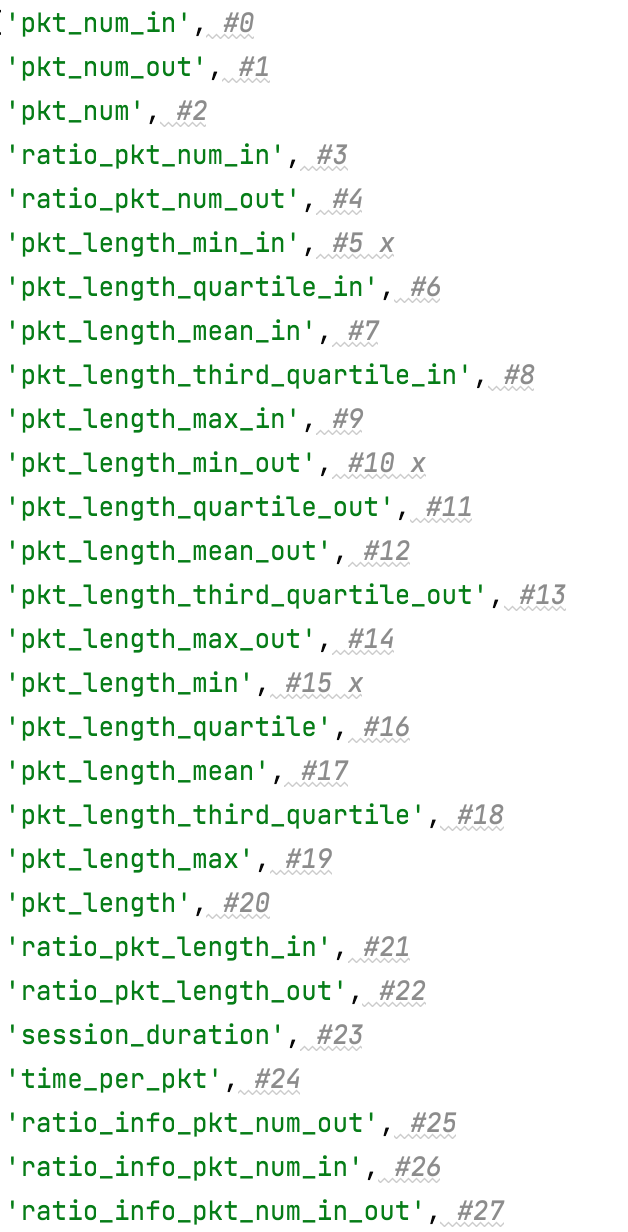
\includegraphics[width=0.5\textwidth]{fig/feature}
    \caption{Features of network traffic data that are being used to train}
    \label{fig:feature}
\end{figure}

Execution example: 
\begin{enumerate}
  \item put the observation1 and observation2 folder into traces folder.
  \item cd to directory A0245095B.
  \item run ./test.sh ../traces/observation1 ../traces/observation2 (It is okay to change '../traces/observationX' to absolute path)
  \item get result.txt in A0245095B folder.
\end{enumerate}


\begin{figure}[h]
    \centering
    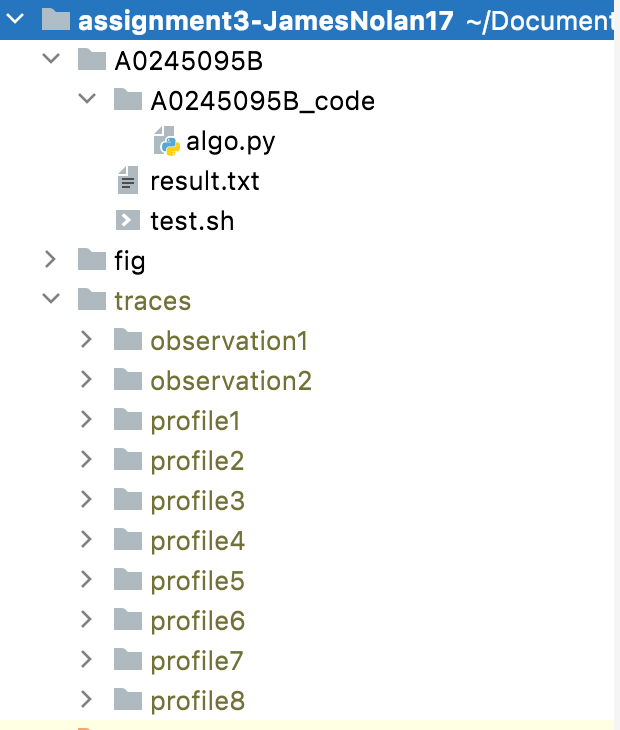
\includegraphics[width=0.5\textwidth]{fig/code}
    \caption{Code Structure}
    \label{fig:code structure}
\end{figure}

Sitation: 


Iterative-Tuning Support Vector Machine For Network Traffic Classification


Machine Learning for Traffic Analysis: A Review



\end{document}
